\documentclass{scu-thesis}
\usepackage[pdftex]{graphicx}	% for including graphics
\usepackage{amsmath}	% for advanced typesetting of mathematics
\usepackage{txfonts}	% for using the Times-Roman font
\usepackage{natbib}		% for better citation styles
\usepackage{placeins}
\usepackage{emp}
\usepackage{ifpdf,graphicx}
\ifpdf
  \DeclareGraphicsRule{*}{mps}{*}{}
\fi
\usepackage{usecases}
\begin{empfile}
\begin{empcmds}
input metauml;
\end{empcmds}

\begin{empdef}[usecasediag](500,500)
  Actor.user("User");

  Usecase.create("Create Project");
  Usecase.add("Add", "Team Members");
  Usecase.assign("Create &", "Assign Tasks");

  add.w = user.human.e + (10,0);

  create.s = add.n + (0,10);
  assign.n = add.s - (0,10);
  
  
  drawObjects(user, add, create, assign);
  clink(association)(user.human, create);
  clink(association)(user.human, add);
  clink(association)(user.human, assign);
\end{empdef}

\begin{empdef}[activityR1](500,500)
Begin.b;
Activity.name("Name Project");
Fork.fork("h", 50);
Activity.define("Define project goal");
Activity.deadline("Define project deadline");
Fork.join("h", 50);
Branch.membAdd;
Activity.addProj("Add people to the project");
End.e;

leftToRight.top(10)(define, deadline);
Group.defineListen(define, deadline);
leftToRight(50)(membAdd, addProj);
topToBottom(20)(b, name, fork, defineListen, join, membAdd, e);



drawObjects(b, name, fork, defineListen, join, membAdd, addProj, e);

clink(transition)(b, name);
clink(transition)(name, fork);
clink(transition)(fork, define);
clink(transition)(fork, deadline);
clink(transition)(define, join);
clink(transition)(deadline, join);
clink(transition)(join, membAdd);
clink(transition)(join, membAdd);
link(transition)(pathStepX(membAdd.e, addProj.n, 0));
link(transition)(pathStepX(addProj.s, e.e, 0));
clink(transition)(membAdd, e);

item(iGuard)("add members")(obj.sw = membAdd.e);
item(iGuard)("done")(obj.nw = membAdd.s + (0, -4));
\end{empdef}

\begin{empdef}[activityR2](500,500)
Begin.be;
Activity.tName("Enter team description");
Branch.addMem;
Activity.contact("Enter member contact");
Branch.cFound;
Activity.addToTeam("Add member to team");
Activity.invite("Send email invite");
Branch.cFoundJoin;
Branch.isLead;
Activity.assProj("Assign project lead role");
Branch.isLeadJoin;
Activity.submit("Submit Team");
End.en;
assProj.midx = invite.midx;
leftToRight.top(25)(addToTeam, invite);
topToBottom(20)(be, tName, addMem, contact, cFound, addToTeam, cFoundJoin, isLead, isLeadJoin, submit, en);
assProj.top = isLead.bottom;


drawObjects(be, tName, addMem, contact, cFound, addToTeam, invite, cFoundJoin, isLead, assProj, isLeadJoin, submit, en);

clink(transition)(be, tName);
clink(transition)(tName, addMem);
clink(transition)(addMem, contact);
link(transition)(pathStepX(cFound.e, invite.n, invite.midx - cFound.width));
clink(transition)(contact, cFound);
link(transition)(pathStepX(invite.s, cFoundJoin.e, 0));
clink(transition)(cFound, addToTeam);
clink(transition)(addToTeam, cFoundJoin);
clink(transition)(cFoundJoin,isLead);
link(transition)(pathStepX(isLead.e, assProj.n, assProj.midx - isLead.width));
link(transition)(pathStepX(assProj.s, isLeadJoin.e, 0));
clink(transition)(isLead, isLeadJoin);
clink(transition)(isLeadJoin, submit); 
clink(transition)(submit, en);
link(transition)(pathStepX(cFoundJoin.w, addMem.w, -60));

item(iGuard)("add members")(obj.nw = addMem.s + (0, -5));
item(iGuard)("contact found")(obj.nw = cFound.s + (0, -5));
item(iGuard)("contact not found")(obj.sw = cFound.e + (10, 0));
item(iGuard)("member is not lead")(obj.nw = isLead.s + (0, -5));
item(iGuard)("member is lead")(obj.sw = isLead.e + (20, 0));
item(iGuard)("done")(obj.nw = isLeadJoin.s + (0, -5));
item(iGuard)("not done")(obj.se = cFoundJoin.w + (-10, 0));
\end{empdef}

\begin{empdef}[activityR4](500,500)
Begin.beg;
Activity.task("Select task");
Activity.selectAss("Select members to assign");
Activity.saveT("Save task");
End.fin;

topToBottom(20)(beg, task, selectAss, saveT, fin);

drawObjects(beg, task, selectAss, saveT, fin);

clink(transition)(beg, task);
clink(transition)(task, selectAss);
clink(transition)(selectAss, saveT);
clink(transition)(saveT, fin);
\end{empdef}

\begin{empdef}[erdiag](500,500)

Class.L("Leader")()();
Class.P("Projects")()();
Class.C("Teams")()();
Class.T("Tasks")()();
Class.M("Members")()();

leftToRight(150)(P, C);
leftToRight(150)(T, M);

Group.PT(P, C);
Group.TM(T, M);

topToBottom(40)(L, PT, TM);



drawObjects(L, PT, TM);

clink(association)(P, C);
item(iAssoc)("1")(obj.sw = P.e);
item(iAssoc)("1..*")(obj.se = C.w);
item(iAssoc)("composed of")(obj.s =.5[P.e,C.w]);

clink(association)(T, M);
item(iAssoc)("1")(obj.sw = T.e);
item(iAssoc)("1..*")(obj.se = M.w);
item(iAssoc)("complete")(obj.s =.5[T.e,M.w]);

link(association)(pathStepX(P.s, T.n, 0));
item(iAssoc)("1")(obj.ne = P.s - (10, 0));
item(iAssoc)("1..*")(obj.se = T.n - (7, 0));
item(iAssoc)("list")(obj.e =.5[P.s,T.n] - (5, 0));

link(association)(pathStepX(C.s, M.n, 0));
item(iAssoc)("1")(obj.nw = C.s + (6, 0));
item(iAssoc)("1..*")(obj.sw = M.n + (8, 0));
item(iAssoc)("have")(obj.w =.5[C.s,M.n] + (10, 0));

link(association)(pathStepX(L.w, P.n, P.midx));
item(iAssoc)("1")(obj.se = L.w);
item(iAssoc)("1..*")(obj.se = P.n);
item(iAssoc)("makes")(obj.e =.5[L.e,P.w] + (-10, 10));

link(association)(pathStepX(L.e, C.n, C.midx - L.width));
item(iAssoc)("1")(obj.sw = L.e);
item(iAssoc)("1..*")(obj.sw = C.n);
item(iAssoc)("guides")(obj.s =.5[L.e,C.w] + (10, 10));

\end{empdef}

\end{empfile}

% These must be set first ... the rest of the thesis commands rely on them.

\author{Alberto Diaz-Tostado}
\author{Amy Nguyen Tran}
\title{Project Management Application}
\department{Department of Computer Science and Engineering}
\degree{Bachelor of Science in Computer Science and Engineering}
\degree{Bachelor of Science in Web Design and Engineering}

% Only bachelor's theses should have multiple authors and/or be from
% multiple departments.  Signatures required:
%
% Bachelor's theses: advisor(s), department chair(s)
% Master's theses: advisor, reader, department chair
% Doctoral theses: doctoral committee (including advisor), department chair

\begin{document}
\frontmatter
\signature{Thesis Advisor}
\signature{Department Chair}

\maketitle
\begin{abstract}
Individuals currently live in a society that revolves around productivity. People from managers to students are bombarded with numerous tasks and daunting deadlines, making it extremely difficult to stay organized. In addition, these individuals also have multiple commitments in their lives, adding to the stress of keeping up with their already busy schedules. Currently, people are faced with a variety of organization methods. However, the two tools most people resort to, e-mail and notepad, have become a burden to organize over time. In addition, current project management solutions are targeted towards large enterprises and not accessible for the general public. We propose a simple and user-friendly web-based solution that will be accessible to all. With the creation of a collaborative project management application, we will allow users to host a collaborative environment by providing them with a web based interface where they can easily communicate with their team members, find an organized list of their tasks and keep track of their project progress. 
\end{abstract}


\tableofcontents
\listoffigures

\mainmatter
\chapter{Introduction}

\section{Motivation}

Individuals currently live in a society that revolves around productivity. People from managers to students are bombarded with numerous tasks and daunting deadlines, making it extremely difficult to stay organized. In addition, people have multiple commitments in their lives, adding to the stress of keeping up with their already busy schedules. Currently, individuals are faced with a variety of organization methods. However, the two tools most people resort to are e-mail and notepads. Without a doubt, people are often drawn to the simplicity of typing out a quick note or sending an e-mail. However, it becomes extremely difficult to keep track of all these notes and e-mails. Before you know it, lines of communication become broken and trains of thought are lost forever. Older conventions are becoming outdated as e-mail searches often yield innumerable results, and text files are never where they need to be. Team members need a way arrange their tasks and project managers require a solution to view the process of projects and ensure that every member is on track. 

\section{Current Solutions} 

Previous solutions have failed to provide an accessible and simple project management tool. One crucial issue is that most workflow management solutions, such as Asana and Basecamp, are often marketed and catered to large enterprises rather students and small groups.These solutions are exceedingly expensive, thus community organizations and students tend to avoid these applications. Another issue with current solutions is their steep learning curves that often require additional training. In addition, present solutions, such as Pivotal Tracker and Microsoft Outlook, are not straightforward and can make it difficult to setup a meeting or look up a contact. Furthermore, present project management applications are visually unappealing and not user-friendly. Most applications follow the conventional three panel layout, as seen in Outlook, pushing your tasks into some sidebar crevice where these tasks can easily be overlooked. These applications are not designed for students or small groups with minimal project management experience.

\section{Proposed Solution}

We propose a simple, yet powerful, web-based solution that lives entirely within a browser. The goal is to have an easily accessible place for not only small groups of students or professionals to host a collaborative environment, but, we also want individuals to use our system for personal projects. Our accessibility will be achieved through a simple sign-on system without the hassle of painful payment systems and complex learning curves. Instead of struggling to learn the software, the user will be guided through a quick, interactive tutorial where he or she will establish goals, deadlines, and other project management tasks. The user will then be able to begin collaborating by creating groups and inviting other team members. Here, the user has the ability to add deadlines as well as assign internal tasks for him/herself or external tasks for others to view. The application will include a progress bar showing where the project is, where it was, and most importantly, where it needs to go. Current solutions provide users with a static page of checklists. In our application, when progress is made, the interface will reflect those changes. The timeline will expand into greater detail, time sensitive reports will become available, and completed tasks and files will be, literally, lost in time.  We will allow the user to travel through their project timeline, revealing a snapshot of previous or future tasks. Lastly, to further promote organization, we plan to allow teams to store files within their project portals, eliminating time spent searching for important documents. Our product will be tested in live working environments, showing how teams use our solution to better organize their projects in an effort to help us help them achieve their organizational goals. 

\chapter{Design}

\section{Conceptual Model}

\subsection{State Diagram}
\begin{figure}[ht]
\centering
\empuse{erdiag}
\caption{Entity Relationship Diagram}
\end{figure}
\FloatBarrier

\subsection{Activity Diagrams}

\begin{figure}[ht]
\centering
\empuse{activityR1}
\caption{Activity Diagram: Creating a project.}
\end{figure}


\begin{figure}[ht]
\centering
\empuse{activityR2}
\caption{Activity Diagram: Creating a team.}
\end{figure}


\begin{figure}[ht]
\centering
\empuse{activityR4}
\caption{Activity Diagram: Assigning tasks.}
\end{figure}
\FloatBarrier

\subsection{Mockups}

\begin{figure}[ht]
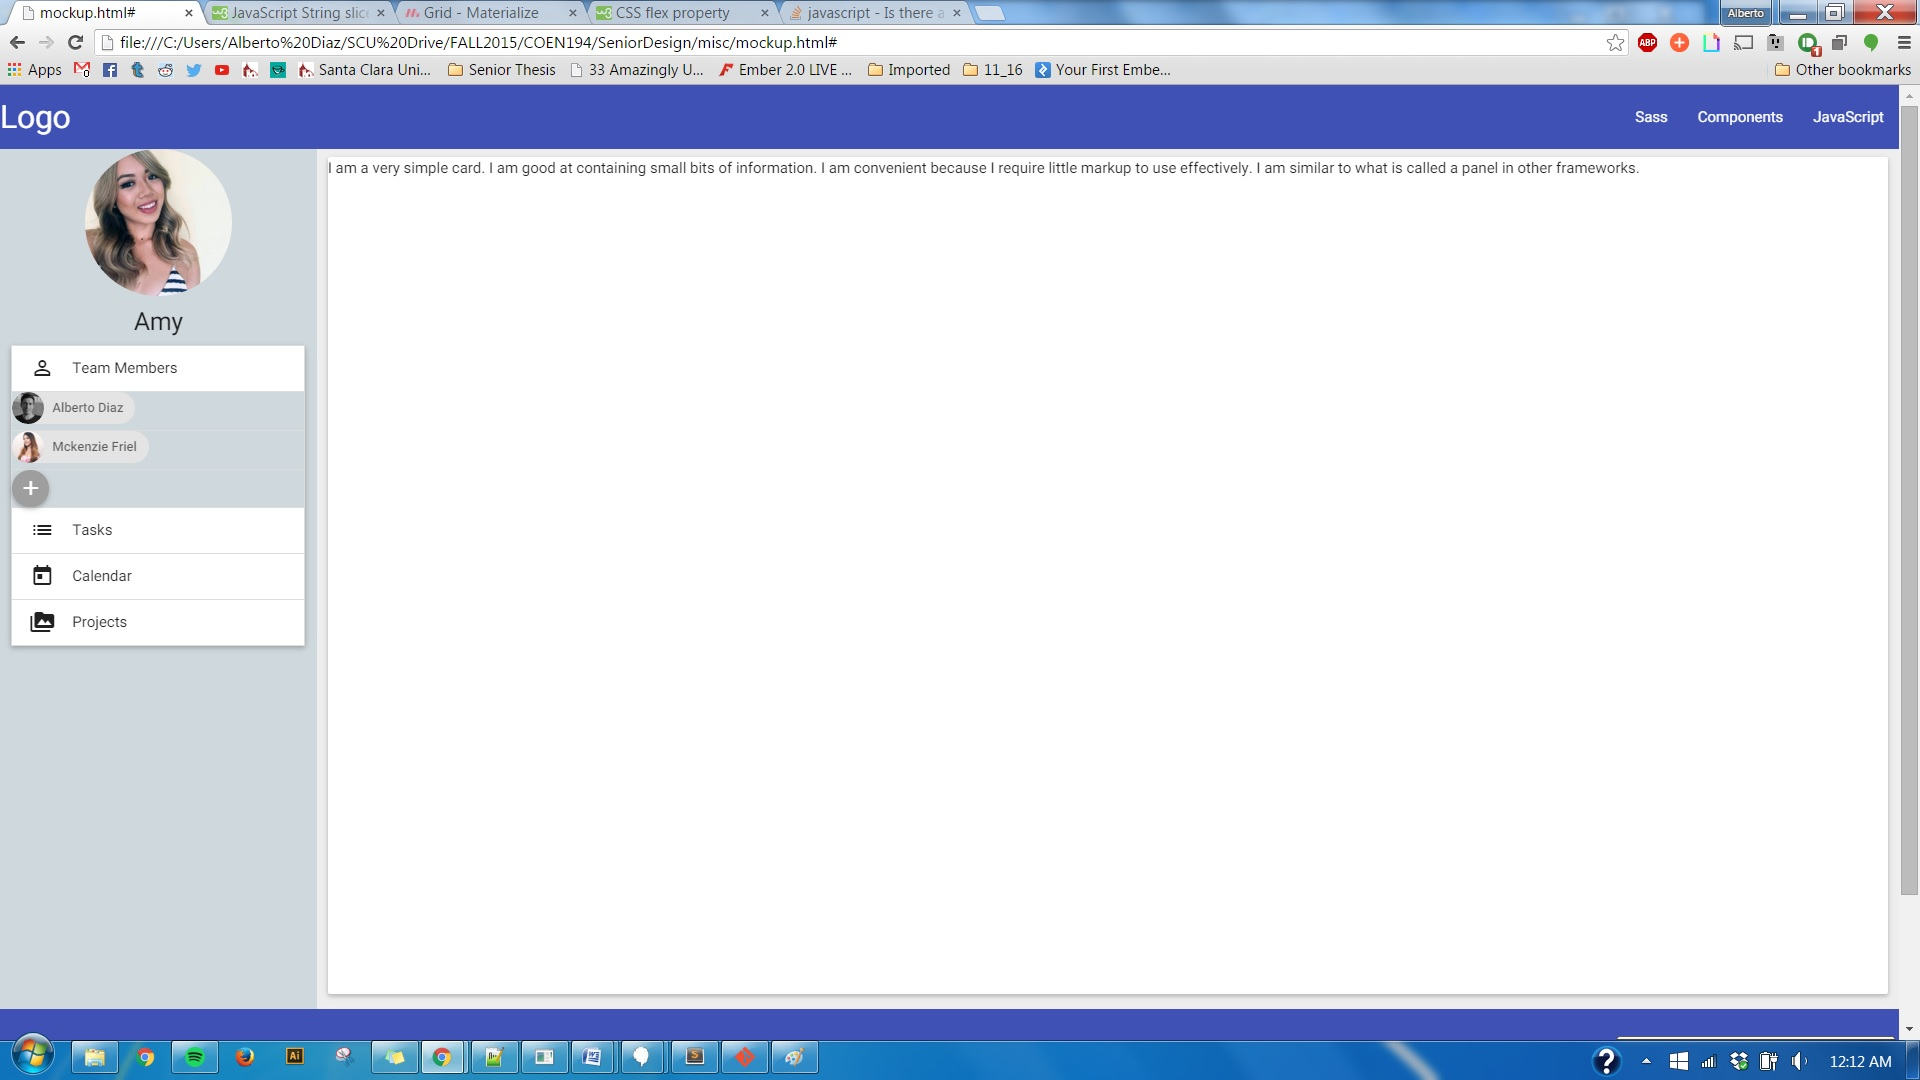
\includegraphics[width=\textwidth]{mockup.jpg}
\caption{A mockup of our system concept.}
\end{figure}
\FloatBarrier

\section{Use Cases}

\begin{figure}[ht]
\centering
\empuse{usecasediag}
\caption{Use Case Diagram}
\end{figure}

\begin{figure}[ht]
\begin{usecase}

\addtitle{Use Case 1}{Create Project} 

\addfield{Goal:}{Initialize project objectives, tasks, and deadlines}

\addfield{Actor:}{User}

\addfield{Preconditions:}{Account is set up}
%when multiple
%\additemizedfield{Preconditions:}{} 

\addfield{Postconditions:}{Project is initialized}
%when multiple
%\additemizedfield{Preconditions:}{}

%Main Success Scenario: A typical, unconditional happy path scenario of success.
\addscenario{Steps:}{
  \item Name the project
  \item Define project goals and deadlines
  \item Add people to the project
  \item Save the project
}

%Extensions: Alternate scenarios of success or failure.
\addscenario{Exceptions:}{
  \item[A.] Invalid login data:
    \begin{enumerate}
    \item[1.] System shows failure message
    \item[2.] User returns to step 1
    \end{enumerate}
  \item[B.] Invalid subsriber data:
    \begin{enumerate}
    \item[1.] System shows failure message
    \item[2.] User returns to step 2 and corrects the errors
    \end{enumerate}
}
\end{usecase}
\end{figure}
\begin{figure}[ht]
\begin{usecase}

\addtitle{Use Case 1}{Template test} 

\addfield{Goal:}{System-wide}

\addfield{Actor:}{End-User}

\addfield{Preconditions:}{}
%when multiple
%\additemizedfield{Preconditions:}{} 

\addfield{Postconditions:}{}
%when multiple
%\additemizedfield{Preconditions:}{}

%Main Success Scenario: A typical, unconditional happy path scenario of success.
\addscenario{Steps:}{
  \item The first action
  \item The second action
}

%Extensions: Alternate scenarios of success or failure.
\addscenario{Exceptions:}{
  \item[2.a] Invalid login data:
    \begin{enumerate}
    \item[1.] System shows failure message
    \item[2.] User returns to step 1
    \end{enumerate}
  \item[5.a] Invalid subsriber data:
    \begin{enumerate}
    \item[1.] System shows failure message
    \item[2.] User returns to step 2 and corrects the errors
    \end{enumerate}
}
\end{usecase}
\end{figure}
\begin{figure}[ht]
\begin{usecase}

\addtitle{Use Case 1}{Template test} 

\addfield{Goal:}{System-wide}

\addfield{Actor:}{End-User}

\addfield{Preconditions:}{}
%when multiple
%\additemizedfield{Preconditions:}{} 

\addfield{Postconditions:}{}
%when multiple
%\additemizedfield{Preconditions:}{}

%Main Success Scenario: A typical, unconditional happy path scenario of success.
\addscenario{Steps:}{
  \item The first action
  \item The second action
}

%Extensions: Alternate scenarios of success or failure.
\addscenario{Exceptions:}{
  \item[2.a] Invalid login data:
    \begin{enumerate}
    \item[1.] System shows failure message
    \item[2.] User returns to step 1
    \end{enumerate}
  \item[5.a] Invalid subsriber data:
    \begin{enumerate}
    \item[1.] System shows failure message
    \item[2.] User returns to step 2 and corrects the errors
    \end{enumerate}
}
\end{usecase}
\end{figure}
\FloatBarrier

\section{Architectural Design}
\begin{figure}[ht]
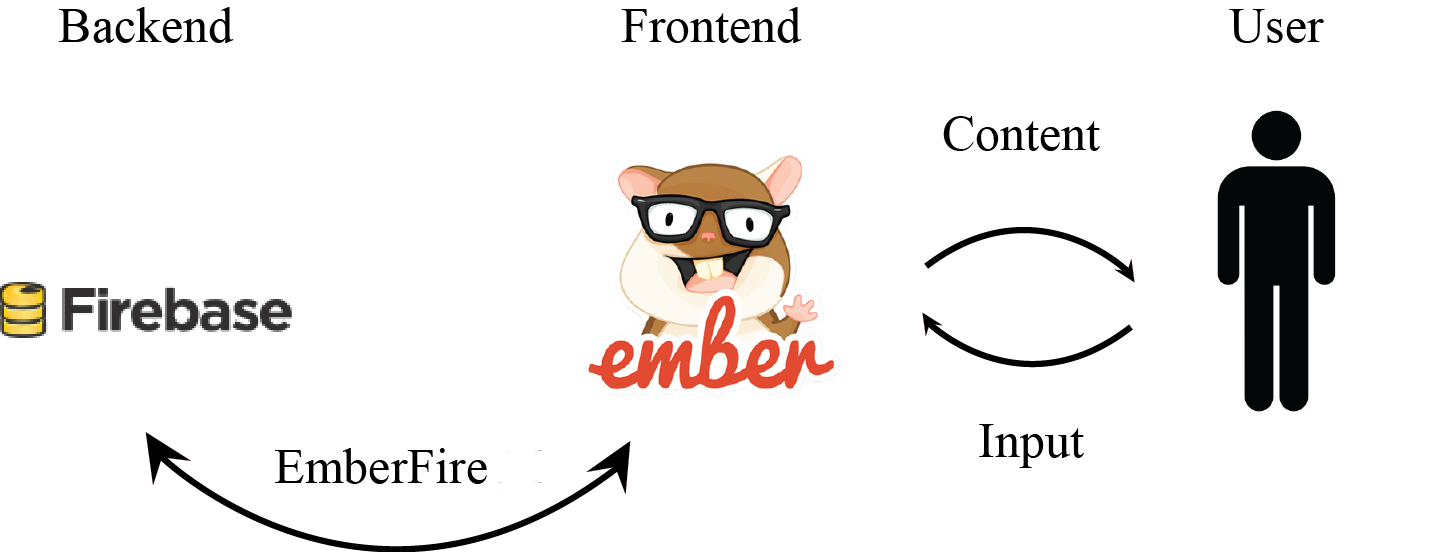
\includegraphics[width=\textwidth]{archDiag.png}
\caption{Diagram describing the technology stack for our application.}
\end{figure}
\FloatBarrier

\section{Technologies Used}
In this section, we describe the technologies we chose to develop our application and the features they provide for us.
\begin{enumerate}
\item HTML5 \par The latest version of the standard web markup language
\item JS \par A high-level, untyped, and interpreted programming  language supported by all modern web browser
\item CSS3 \par A stylesheet language used to describe the presentation of HTML documents
\item Ember.js \par A front-end javascript framework based on the model-view-controller (MVC) model and applies programming conventions to build scalable applications
\item  Firebase \par A backend-as-a-service that provides client-side APIs, and services such as databases, web hosting, and authentication.
\end{enumerate}

\section{Design Rationale}
In this section, we describe why we chose these technologies and the advantages and disadvantages associated with each of those technologies. 
\begin{enumerate}
\item HTML5/CSS3 /JS \par The latest version of the standard web markup language
	\begin{enumerate}
	
	\end{enumerate}
\item Ember.js \par A front-end javascript framework based on the model-view-controller (MVC) model and applies programming conventions to build scalable applications
\item  Firebase \par A backend-as-a-service that provides client-side APIs, and services such as databases, web hosting, and authentication.
\end{enumerate}

\backmatter
\immediate\write18{mpost -tex=latex \jobname}
\end{document}
